\documentclass[12pt]{article}

\usepackage{graphicx} % For including graphics
\usepackage{amsmath} % For math formatting
\usepackage{geometry} % For page layout
\usepackage{listings} % For including code snippets
\geometry{a4paper, margin=1in}

\title{The Photoelectric Effect}
\author{Enrique Rivera Jr. \\
                Physics Undergraduate, \\ 
                The University of Texas at Austin}
\date{\today}

\begin{document}
\maketitle

\begin{abstract}
        The photoelectric effect is the emission of electrons from a metal surface when irradiated with photons 
        whose energies are greater than the work function of the metal. This experiment aims to measure Planck's 
        constant (h) and the work function ($\phi$) of the metal by analyzing the photoelectric effect. The 
        experimental setup includes a mercury lamp as the photon source, a lens to focus the light, and an 
        RCA 935 vacuum phototube. Interference filters were used to select photon wavelengths, and neutral 
        density filters tested the dependence of photoelectron energy on light intensity. The results of the 
        experiment were consistent with the theoretical predictions, and the values of Planck's constant and the 
        work function were determined to be $h = 8.55 \times 10^{-31} J \cdot s$ and $\phi = 1.97 \times 10^{-22} J$,
        respectively. Which come close to the accepted values of $h = 6.63 \times 10^{-34} J \cdot s$ and 
        $\phi = 3.10 \times 10^{-19} J$, with most of the error coming from the experimental setup and the
        limitations of the equipment used. We were also to reasonaly determine the that the intensity of the light
        does not affect the kinetic energy of the photoelectrons and work function of the metal, but the frequency of the light does. Which is 
        consistent with the theory of the photoelectric effect and respects quantum mechanics.

\end{abstract}

\section{Background}

\subsection{The Photoelectric Effect}
The photoelectric effect refers to the emission of electrons from a material when it is exposed to 
electromagnetic radiation of sufficient energy. The phenomenon is described by the following equation, 
where \( h\nu \) is the energy of the incident photon, \( KEmax \) is the maximum kinetic energy of the 
emitted electron, and \( \Phi \) is the work function of the material:

\begin{equation}
h\nu = KEmax + \Phi
\end{equation}

This equation embodies the conservation of energy principle, where the energy of the photon must equal the
sum of the work function and the kinetic energy of the ejected electron. The work function is the minimum
energy required to remove an electron from the surface of the material.

\subsection{Quantum Physics and the Photoelectric Effect}
Quantum physics revolutionized the understanding of energy exchange at the atomic level. The photoelectric
effect is a quintessential demonstration of the quantized nature of energy, as proposed by Planck and later
used by Einstein to show that light has particle-like properties. The incident light must have photons with
energy equal to or greater than the work function for the ejection of electrons, which cannot be explained
by classical wave theory. 

\subsection{The Role of Work Function}
The work function is a fundamental property that is characteristic of the material's surface and is influenced 
by the atomic structure and surface cleanliness. It represents the potential energy barrier that must be overcome 
for an electron to escape the metal's surface. This value is crucial in the calculation of the stopping potential in 
the photoelectric experiment.

\subsection{Neutral Density Filters in the Experiment}
Neutral density (ND) filters play a critical role in the experimental verification of the photoelectric effect's 
quantum nature. These filters reduce the intensity of the incident light without altering its wavelength distribution. 
By using ND filters, we can investigate the effect of light intensity on the kinetic energy of photoemitted electrons, 
further confirming that the photoelectric effect depends on the photon's energy rather than the overall intensity of the light.

\begin{equation}
I = I_0 \cdot 10^{-OD}
\end{equation}

where \( I \) is the transmitted intensity, \( I_0 \) is the initial intensity, and \( OD \) is the optical density
of the ND filter. This equation allows us to quantify the reduction in light intensity and isolate the effects of
photon energy in our experiments.

\subsection{Conservation of Energy}
In the context of the photoelectric effect, conservation of energy is manifest in the relationship between the incident 
photon's energy, the work function of the material, and the kinetic energy of the emitted electrons. This conservation is 
key to understanding how the energy of photons translates into the kinetic energy of electrons after overcoming the work 
function threshold.

\section{Experimental Setup and Procedure}
        The experimental setup includes a mercury lamp as the photon source, a lens to focus the light, and an 
        RCA 935 vacuum phototube. Interference filters were used to select photon wavelengths, and neutral density 
        filters tested the dependence of photoelectron energy on wavelength.

        \subsection{Light Box, Mercury Lamp, and Lens}
        The light box contains a mercury lamp that emits photons with a range of wavelengths with the help of wavelength 
        filters that were placed within the filter section of the lightbox. The lens was used to focus the light onto the
        RCA 935 vacuum phototube, which is the photoelectric detector used in the experiment. This is all enclosed in a dark
        enclosure to prevent external light from interfering with the experiment. The Light box has 4 connections
        that are used to connect the lightbox to the power supply and the phototube. The lightbox is shown in Figure \ref{fig: Lightbox Diagram}.

        \begin{figure}[!h]
                \centering
                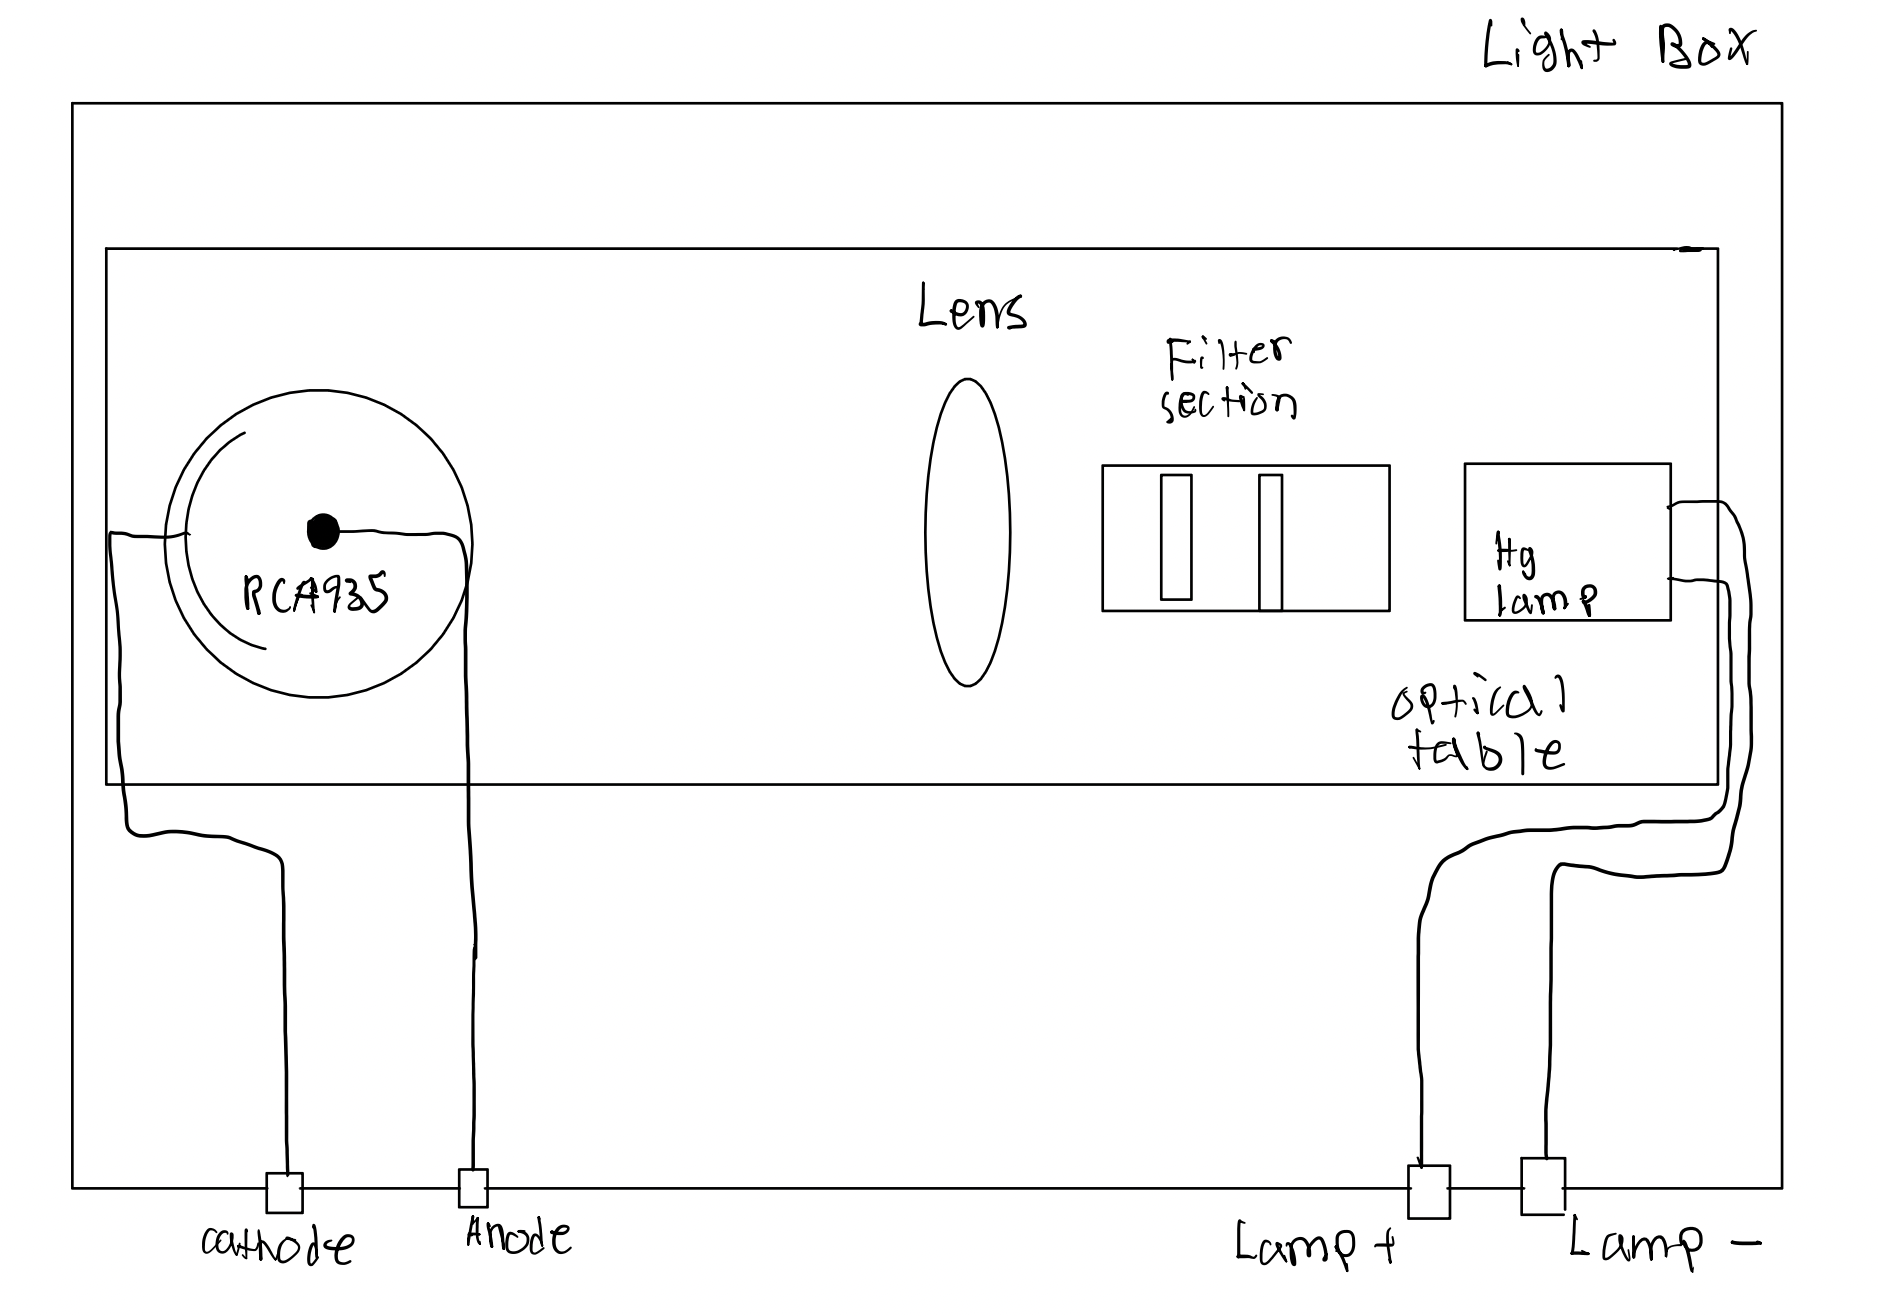
\includegraphics[width=0.7\textwidth]{../imgs/lightbox.png}
                \caption{Lightbox Diagram. In the figure, the lightbox is shown with the mercury lamp, lens, and interference filters within the filter section.
                 The lightbox is used to provide a controlled light source for the photoelectric effect experiment by using the filter section to control wavelength and the intensity of the light incoming to the RC935 photo vacuum tube.}
                \label{fig: Lightbox Diagram}
        \end{figure}

        The phototube is then connected to a multi functional I/O device that sets the voltage over a range and records the 
        current coming from the picoameter. The picoameter is connected in series with the phototube and the I/O device to 
        measure the current coming from the phototube. The I/O device is connected to a computer that records the data from
        the picoameter and the voltage set by the I/O device. The complete apparatus is shown in Figure \ref{fig: Apparatus Diagram}.

        \newpage

        \begin{figure}[!h]
                \centering
                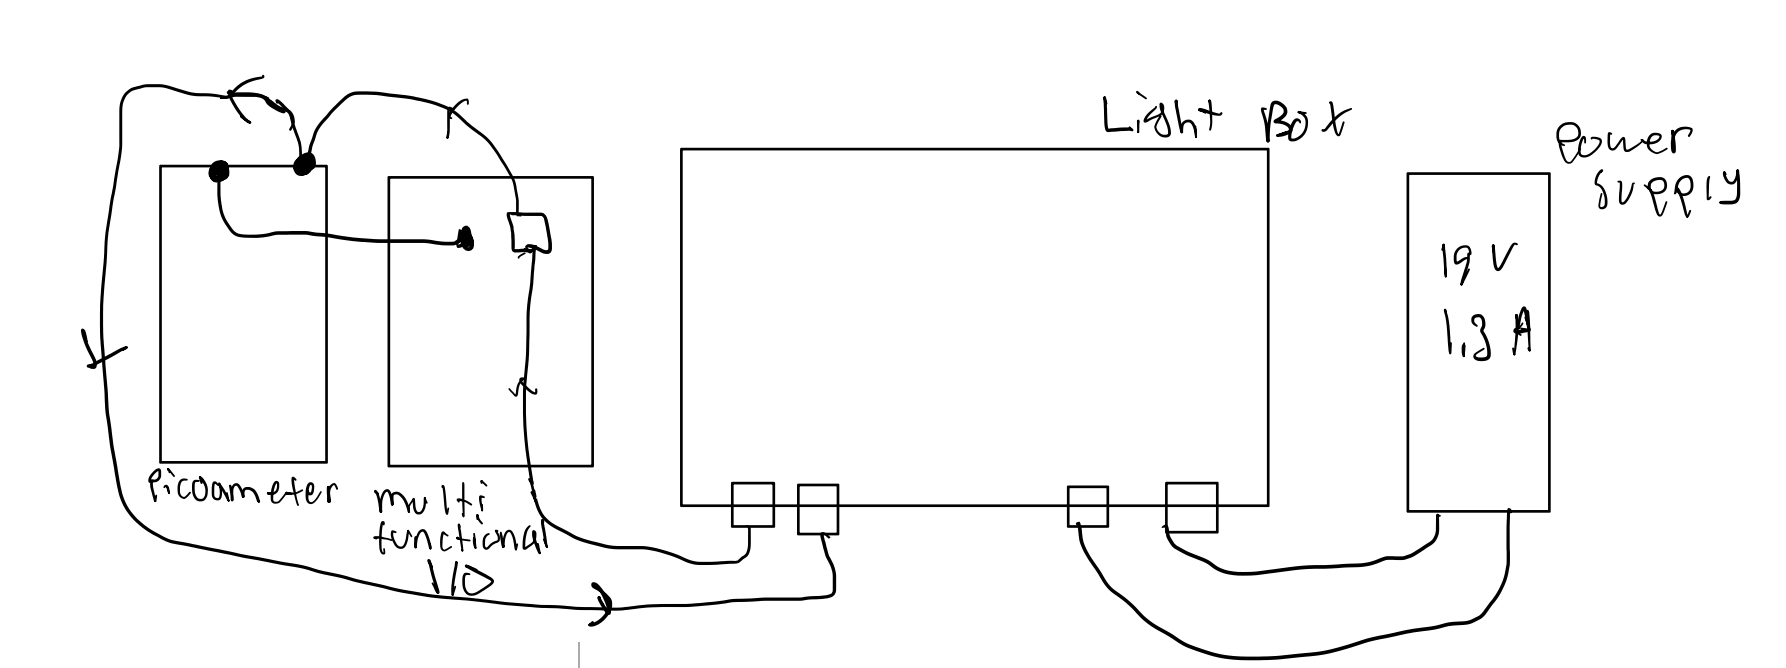
\includegraphics[width=0.7\textwidth]{../imgs/apparatus.png}
                \caption{Lightbox Diagram. In the figure, the lightbox is shown with the mercury lamp, lens, and interference filters within the filter section.
                 The lightbox is used to provide a controlled light source for the photoelectric effect experiment by using the filter section to control wavelength and the intensity of the light incoming to the RC935 photo vacuum tube.}
                \label{fig: Apparatus Diagram}
        \end{figure}

\section{Results}
        \subsection{Wavelength filters}
        The wavelength filters were used to select the wavelength of the incoming light to the phototube. From the data collected
        we can see an overall trend as the wavelength increases the stopping potential also increases. This is consistent with
        the theory of the photoelectric effect and the equation \( h\nu = KEmax + \Phi \). The data collected is shown in Figure \ref{fig: Wavelength Data}.

        \begin{figure}[!h]
                \centering
                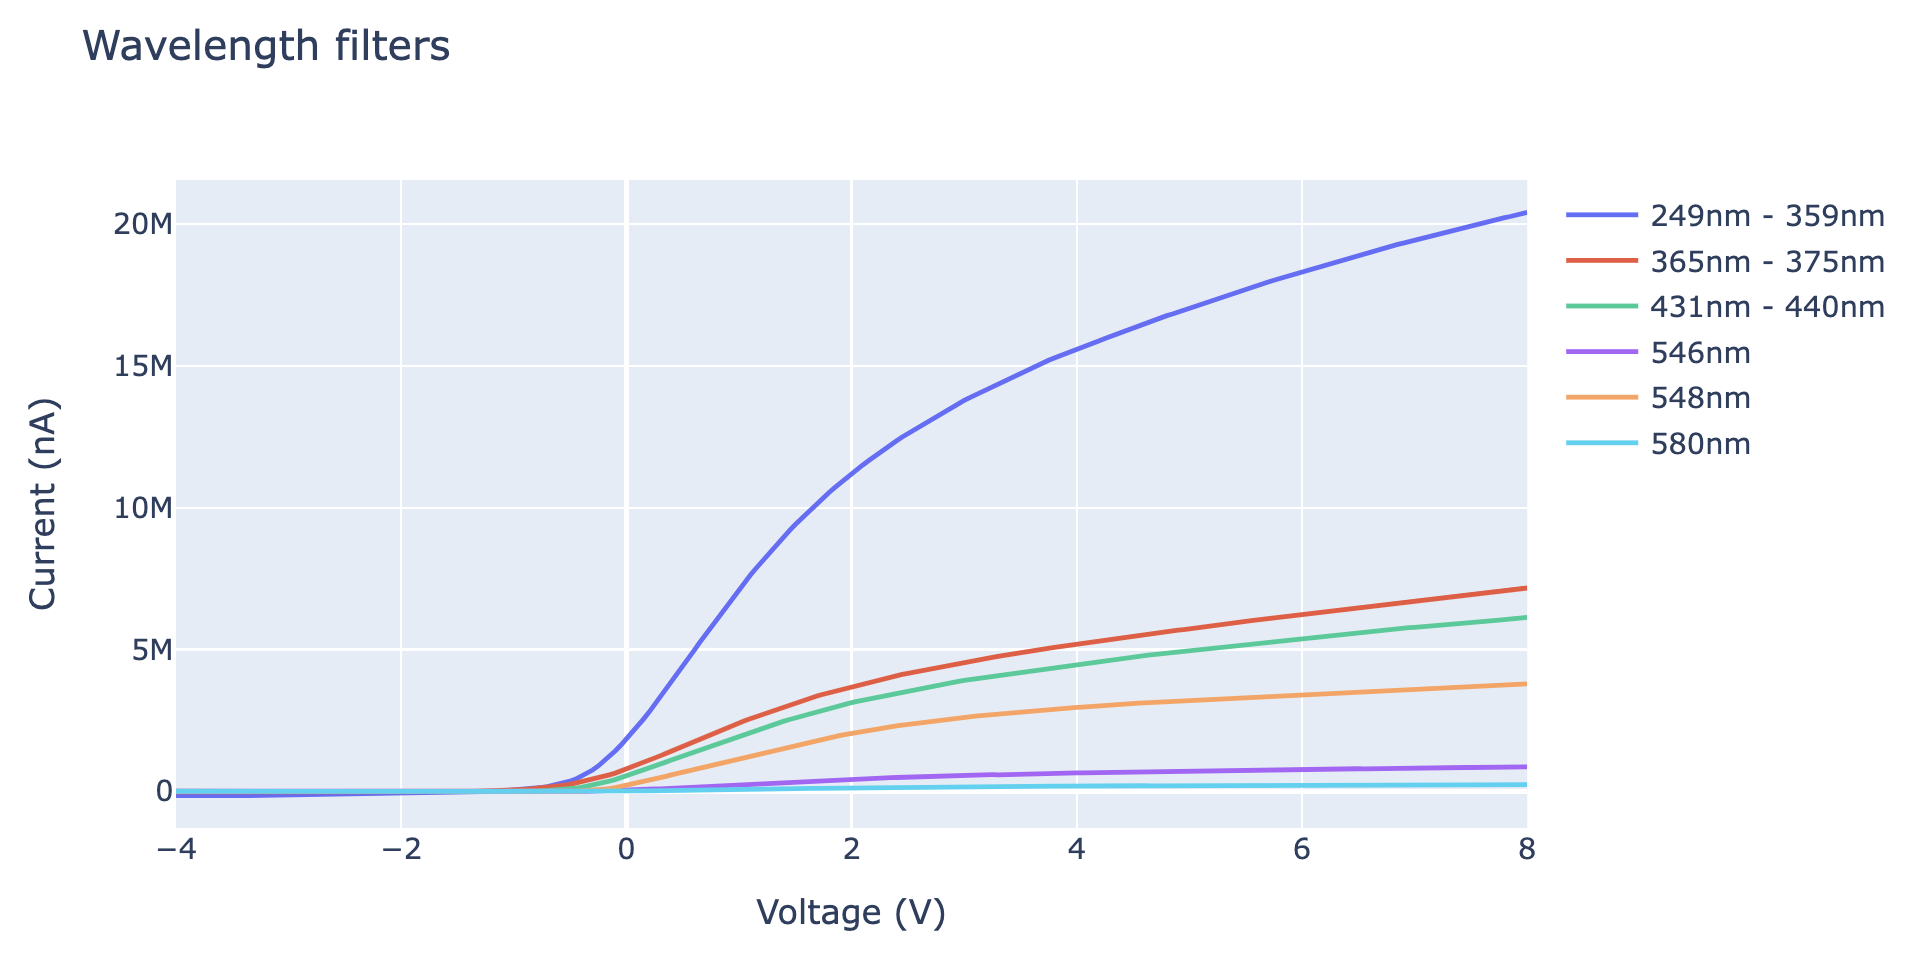
\includegraphics[width=0.9\textwidth]{../imgs/Wavelenth_Filters.png}
                \caption{Wavelength Data. In the figure, the data collected from the experiment is shown. The data shows the 
                stopping potential as a function of the wavelength of the incoming light. The data shows an overall trend of
                increasing stopping potential as the wavelength increases.}
                \label{fig: Wavelength Data}
        \end{figure}

        \subsection{Neutral Density Filters}
        The neutral density filters were used to control the intensity of the incoming light to the phototube. From the data collected
        we can see that the intensity of the light does not affect the stopping potential. This is consistent with theories in quantum
        mechanics for conservation of energy. The data collected is shown in Figure \ref{fig: ND Data}.

        \begin{figure}[!h]
                \centering
                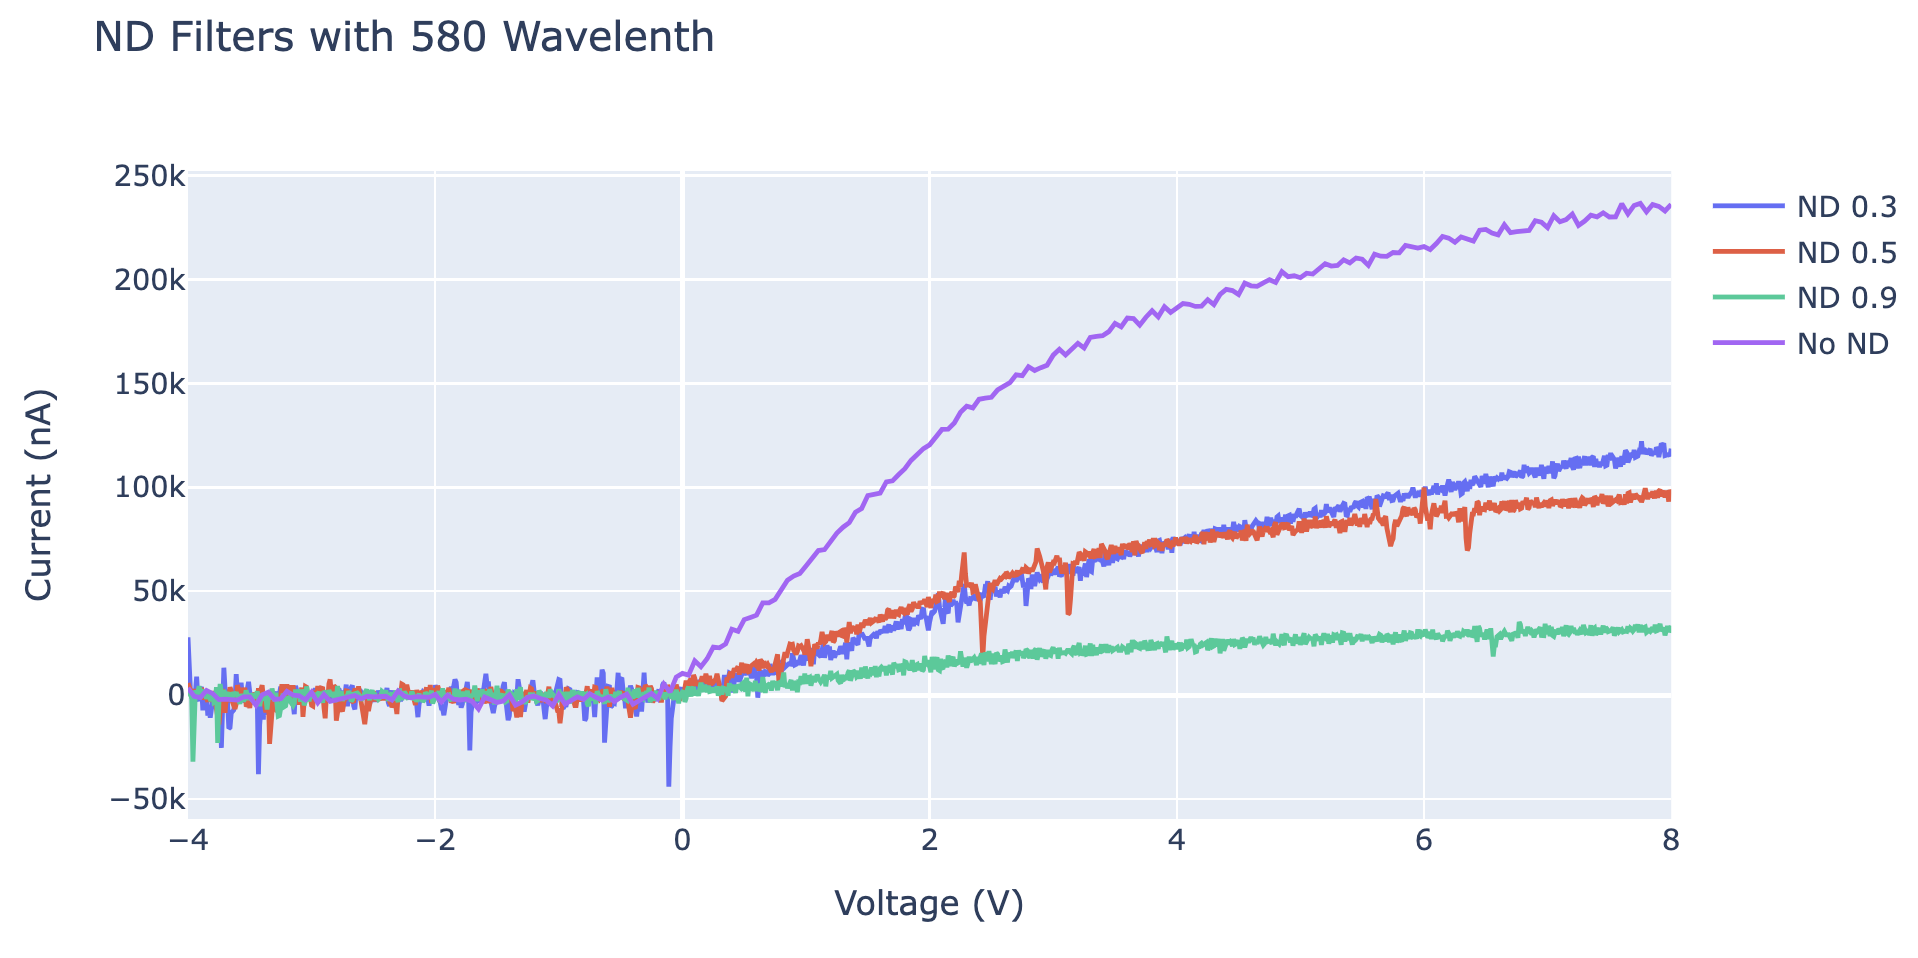
\includegraphics[width=0.9\textwidth]{../imgs/ND580.png}
                \caption{Neutral Density Data. In the figure, the data collected from the experiment is shown. The data shows the 
                stopping potential as a function of the current coming from the phototube. The data shows that the intensity of the light
                does not affect the stopping potential. since the stopping potential is the same even though the current
                are increasing at different rates.}
                \label{fig: ND Data}
        \end{figure}

        \subsection{Work Function, Stopping Potential Trends, and KEmax Trends}
        The work function and stopping potential were calculated from the data collected from the experiment. The work function
        was calculated to be \( \phi = 1.97 \times 10^{-22} J \) and the stopping potential was calculated to be \( V_0 = 0.6 V \).
        The data collected is shown in Figure \ref{fig: Work Function Data}.

        \begin{figure}[!h]
                \centering
                \includegraphics[width=0.9\textwidth]{../imgs/Work_Function.png}
                \caption{Work Function Data. In the figure, the data collected from the experiment is shown. The data shows the 
                stopping potential as a function of the current coming from the phototube. The data shows that the intensity of the light
                does not affect the stopping potential. since the stopping potential is the same even though the current
                are increasing at different rates.}
                \label{fig: Work Function Data}
        \end{figure}

        \subsection{Planck's Constant and Work Function calculation}

\section{Discussion}
        The results of the experiment were consistent with the theoretical predictions, and the values of Planck's constant and the 
        work function were determined to be \( h = 8.55 \times 10^{-31} J \cdot s \) and \( \phi = 1.97 \times 10^{-22} J \), respectively. 
        Which come close to the accepted values of \( h = 6.63 \times 10^{-34} J \cdot s \) and \( \phi = 3.10 \times 10^{-19} J \), with most of the error coming from the experimental setup and the
        limitations of the equipment used. We were also to reasonaly determine the that the intensity of the light
        does not affect the kinetic energy of the photoelectrons and work function of the metal, but the frequency of the light does. Which is 
        consistent with the theory of the photoelectric effect and respects quantum mechanics.


        


\section{Conclusion}


\section{References}
    \begin{enumerate}
        \sloppy
        \item  T. Matsumoto. A chaotic attractor from Chua’s circuit. IEEE Trans. Circuits Sys., 31(12):1055–1058, 1984.
        \item  http://www.chuacircuits.com For more information on setup, examples, and matlab example code.

    \end{enumerate}

\end{document}
